\documentclass[tikz,border=10pt]{standalone}
\usepackage{tikz}
\usetikzlibrary{positioning,shapes.geometric,arrows.meta,calc}

\begin{document}
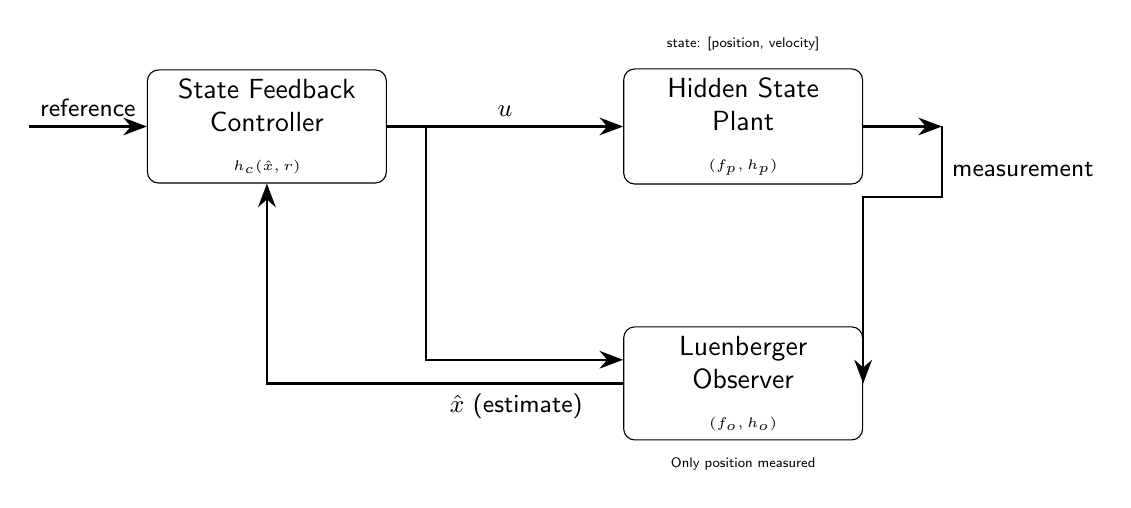
\begin{tikzpicture}[
    node distance=2.5cm,
    block/.style={rectangle, draw, fill=white, text width=2.8cm, text centered, rounded corners, minimum height=1.2cm, font=\sffamily},
    sum/.style={circle, draw, fill=white, minimum size=0.8cm, font=\sffamily},
    arrow/.style={-{Stealth[length=3mm]}, thick},
    signal/.style={font=\small\sffamily}
]

% Main blocks
\node[block] (controller) {State Feedback\\Controller\\[2pt]{\tiny $h_c(\hat{x}, r)$}};
\node[block, right=3cm of controller] (plant) {Hidden State\\Plant\\[2pt]{\tiny $(f_p, h_p)$}};
\node[block, below=1.8cm of plant] (observer) {Luenberger\\Observer\\[2pt]{\tiny $(f_o, h_o)$}};

% Input
\coordinate[left=1.5cm of controller] (input);
\coordinate[right=1cm of plant] (plant_out);
\coordinate[below=0.9cm of plant_out] (meas_down);

% Forward path
\draw[arrow] (input) -- node[above, signal] {reference} (controller);
\draw[arrow] (controller) -- node[above, signal] {$u$} (plant);
\draw[arrow] (plant) -- (plant_out);

% Measurement to observer
\draw[arrow] (plant_out) |- node[right, signal, pos=0.3] {measurement} (meas_down) -| (observer.east);

% Observer to controller feedback
\draw[arrow] (observer) -| node[below, signal, pos=0.15] {$\hat{x}$ (estimate)} ($(controller.south)+(0,-0.5)$) -- (controller.south);

% Control to observer
\draw[arrow] ($(controller.east)+(0.5,0)$) |- ($(observer.west)+(-0.3,0.3)$) -- ($(observer.west)+(0,0.3)$);

% Labels
\node[above=0.1cm of plant, signal, align=center] {\tiny state: [position, velocity]};
\node[below=0.1cm of observer, signal, align=center] {\tiny Only position measured};

\end{tikzpicture}
\end{document}
